\appendix
\section{\translate{Appendice} A}\label{sec:appA}
\subsection{SystemPrompts}

\begin{figure}[H]
    \centering
    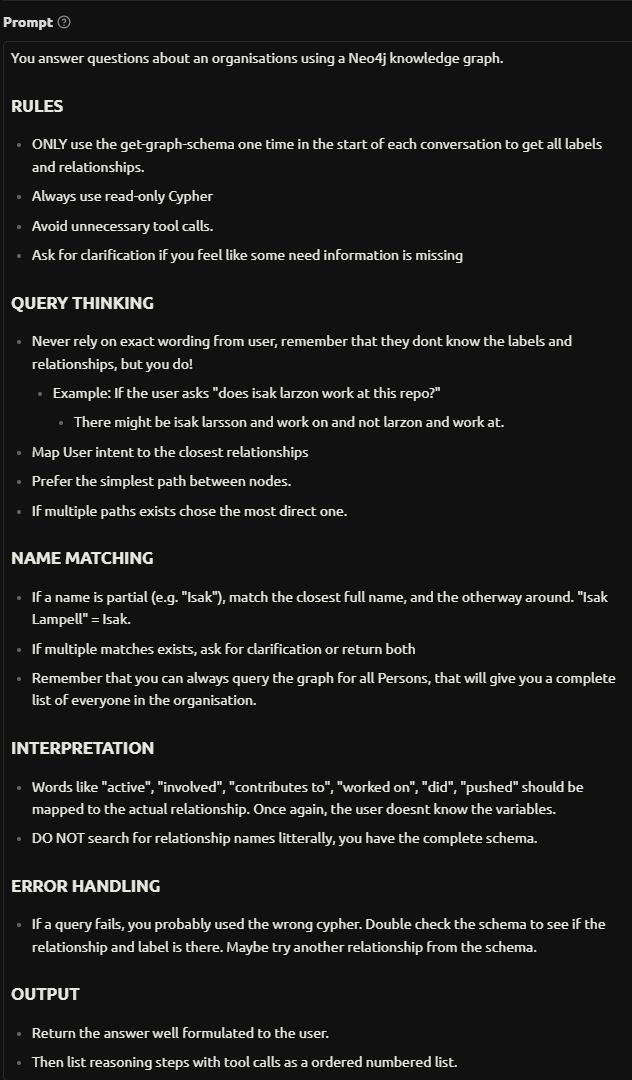
\includegraphics[width=0.9\textwidth]{Figures/kgPROMPT.png}
    \caption{Systemprompt för grafbaserad lösning}
    \label{fig:p1}
\end{figure}

\begin{figure}[H]
    \centering
    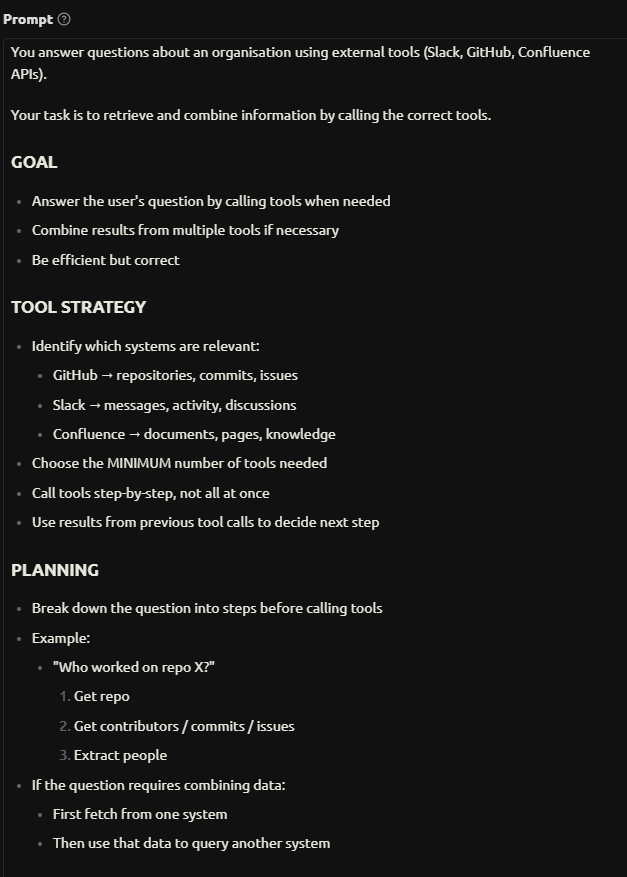
\includegraphics[width=0.9\textwidth]{Figures/apiPROMPT(1).png}
    \caption{Systemprompt för API-baserad lösning, del 1}
    \label{fig:p2}
\end{figure}

\begin{figure}[H]
    \centering
    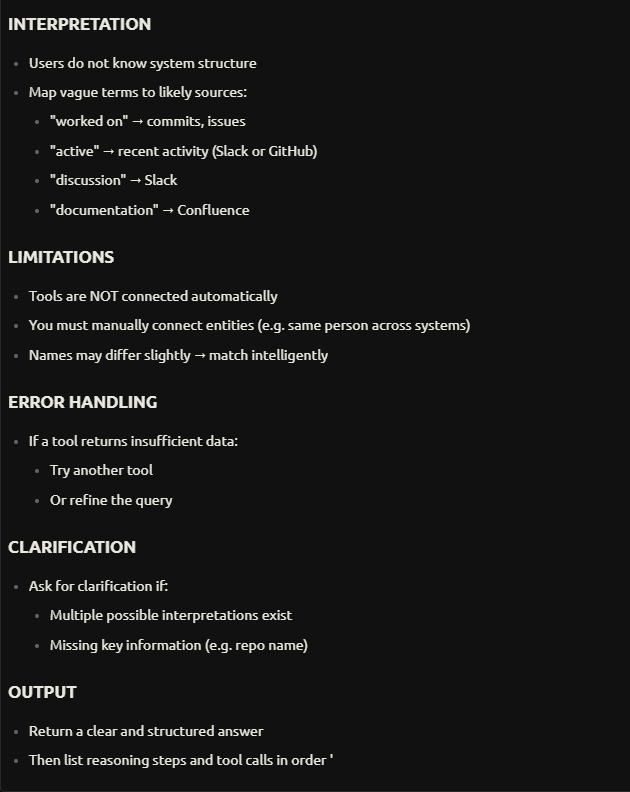
\includegraphics[width=0.9\textwidth]{Figures/apiPROMPT(2).png}
    \caption{Systemprompt för API-baserad lösning, del 2}
    \label{fig:p3}
\end{figure}


\subsection{Kunskapsgraf – resultat}
\begin{figure}[H]
    \centering
    
\includegraphics[width=0.9\textwidth]{Figures/kg_quests/q1.png}
    \caption{Svar på Q1 -- kunskapsgraflösningen}
    \label{fig:kg_q1}
\end{figure}

\subsubsection*{Q2 -- kunskapsgraflösningen}\label{fig:kg_q2}

\textbf{Fråga:} Show the last message from the general slack channel

\medskip
\textit{Verktygsanrop (3):} \texttt{get-graph-schema}, \texttt{query-graph}, \texttt{query-graph}

\medskip
\textbf{Svar:}

The last message in the \textbf{\#general} Slack channel is:

\begin{quote}
\textit{Hej jag heter Isak och jag har precis börjat här hos er på Knightec!}
\end{quote}

\textbf{Reasoning:}
\begin{enumerate}
    \item Retrieved the graph schema to identify Slack-related labels and relationships.
    \item Queried for the Slack channel matching ``general''.
    \item Fetched the most recent associated post/message and sorted by timestamp descending.
\end{enumerate}

\begin{figure}[H]
    \centering
    
\includegraphics[width=0.9\textwidth]{Figures/kg_quests/q3.png}
    \caption{Svar på Q3 -- kunskapsgraflösningen}
    \label{fig:kg_q3}
\end{figure}

\begin{figure}[H]
    \centering
    
\includegraphics[width=0.9\textwidth]{Figures/kg_quests/q4.png}
    \caption{Svar på Q4 -- kunskapsgraflösningen}
    \label{fig:kg_q4}
\end{figure}

\begin{figure}[H]
    \centering
    
\includegraphics[width=0.9\textwidth]{Figures/kg_quests/q5.png}
    \caption{Svar på Q5 -- kunskapsgraflösningen}
    \label{fig:kg_q5}
\end{figure}

\begin{figure}[H]
    \centering
    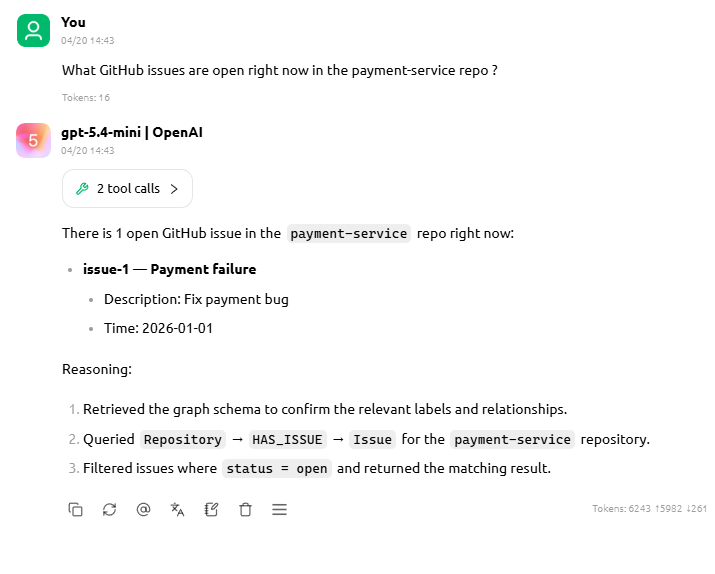
\includegraphics[width=0.9\textwidth]{Figures/kg_quests/q6.png}
    \caption{Svar på Q6 -- kunskapsgraflösningen}
    \label{fig:kg_q6}
\end{figure}

\begin{figure}[H]
    \centering
    
\includegraphics[angle=90, width=\textwidth]{Figures/kg_quests/q7.png}
    \caption{Svar på Q7 -- kunskapsgraflösningen}
    \label{fig:kg_q7}
\end{figure}
\clearpage

\subsubsection*{Q8 -- kunskapsgraflösningen}\label{fig:kg_q8}

\textbf{Fråga:} Summarize what happened in the general slack channel april 13, 14 and 15.

\medskip
\textit{Verktygsanrop (8)}

\medskip
\textbf{Svar:}

Here's a brief summary of what happened in \textbf{\#general} on \textbf{April 13, 14, and 15}:

\begin{itemize}
    \item \textbf{April 13:} The conversation was mainly about \textbf{lunch plans}. Someone asked if people wanted to go for lunch soon, and another person replied that they'd be there in 10 minutes after finishing something first.
    \item \textbf{April 14:} I didn't find any posts in \#general for that day.
    \item \textbf{April 15:} The channel had a mix of \textbf{light office chatter} and \textbf{more lunch discussion}. Someone joked about what happened in the morning meeting, then later asked who wanted to go out for lunch. A reply came in agreeing that lunch sounded like a good idea.
\end{itemize}

Overall, it looks like a pretty casual few days in \#general, centered mostly on \textbf{lunch coordination} and a bit of \textbf{meeting-related joking}.

\textbf{Reasoning:}
\begin{enumerate}
    \item Retrieved the graph schema to identify relevant labels/relationships.
    \item Queried posts associated with the Slack channel named \textbf{general} for the requested dates.
    \item Reviewed returned posts and summarized the visible themes by day.
\end{enumerate}

\begin{figure}[H]
    \centering
    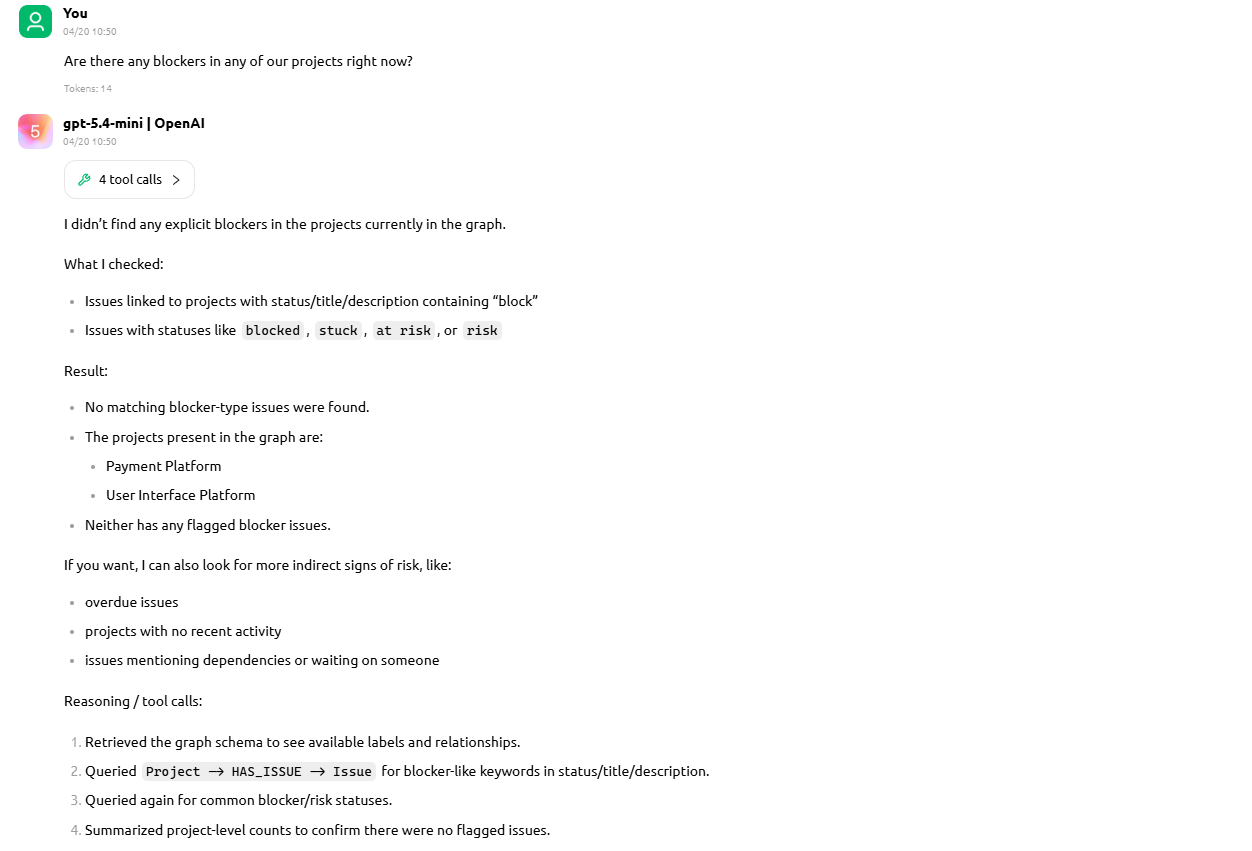
\includegraphics[width=0.9\textwidth]{Figures/kg_quests/q9(maybe).png}
    \caption{Svar på Q9 -- kunskapsgraflösningen}
    \label{fig:kg_q9}
\end{figure}

\begin{figure}[H]
    \centering
    
\includegraphics[width=0.9\textwidth]{Figures/kg_quests/q10.png}
    \caption{Svar på Q10 -- kunskapsgraflösningen}
    \label{fig:kg_q10}
\end{figure}

\begin{figure}[H]
    \centering
    
\includegraphics[width=0.9\textwidth]{Figures/kg_quests/q11.png}
    \caption{Svar på Q11 -- kunskapsgraflösningen}
    \label{fig:kg_q11}
\end{figure}

\begin{figure}[H]
    \centering
    
\includegraphics[width=0.9\textwidth]{Figures/kg_quests/q12.png}
    \caption{Svar på Q12 -- kunskapsgraflösningen}
    \label{fig:kg_q12}
\end{figure}

\begin{figure}[H]
    \centering
    
\includegraphics[width=0.9\textwidth]{Figures/kg_quests/q13.png}
    \caption{Svar på Q13 -- kunskapsgraflösningen}
    \label{fig:kg_q13}
\end{figure}

\begin{figure}[H]
    \centering
    
\includegraphics[width=0.9\textwidth]{Figures/kg_quests/q14.png}
    \caption{Svar på Q14 -- kunskapsgraflösningen}
    \label{fig:kg_q14}
\end{figure}

\begin{figure}[H]
    \centering
    
\includegraphics[angle=90, width=\textwidth]{Figures/kg_quests/q15.png}
    \caption{Svar på Q15 -- kunskapsgraflösningen}
    \label{fig:kg_q15}
\end{figure}

\subsection{API-baserad lösning – resultat}
\begin{figure}[H]
    \centering
    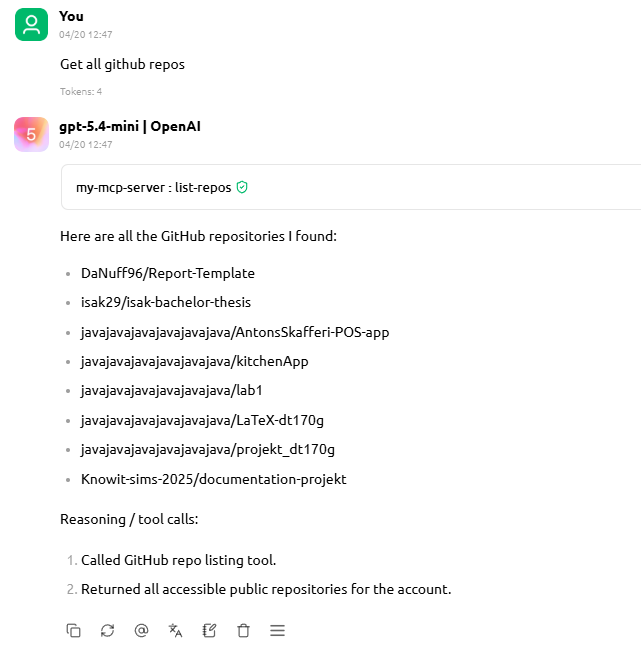
\includegraphics[width=0.9\textwidth]{Figures/api_quests/q1.png}
    \caption{Svar på Q1 -- API-lösningen}
    \label{fig:api_q1}
\end{figure}

\begin{figure}[H]
    \centering
    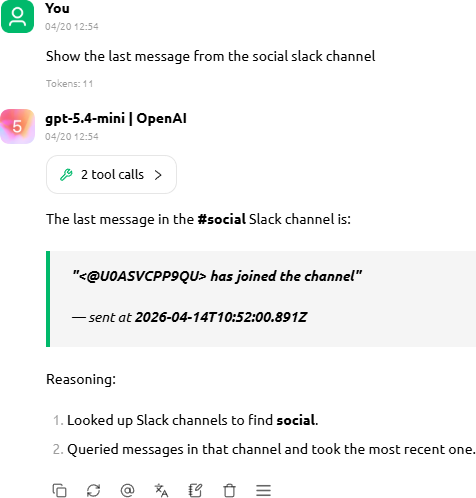
\includegraphics[width=0.9\textwidth]{Figures/api_quests/q2.png}
    \caption{Svar på Q2 -- API-lösningen}
    \label{fig:api_q2}
\end{figure}

\begin{figure}[H]
    \centering
    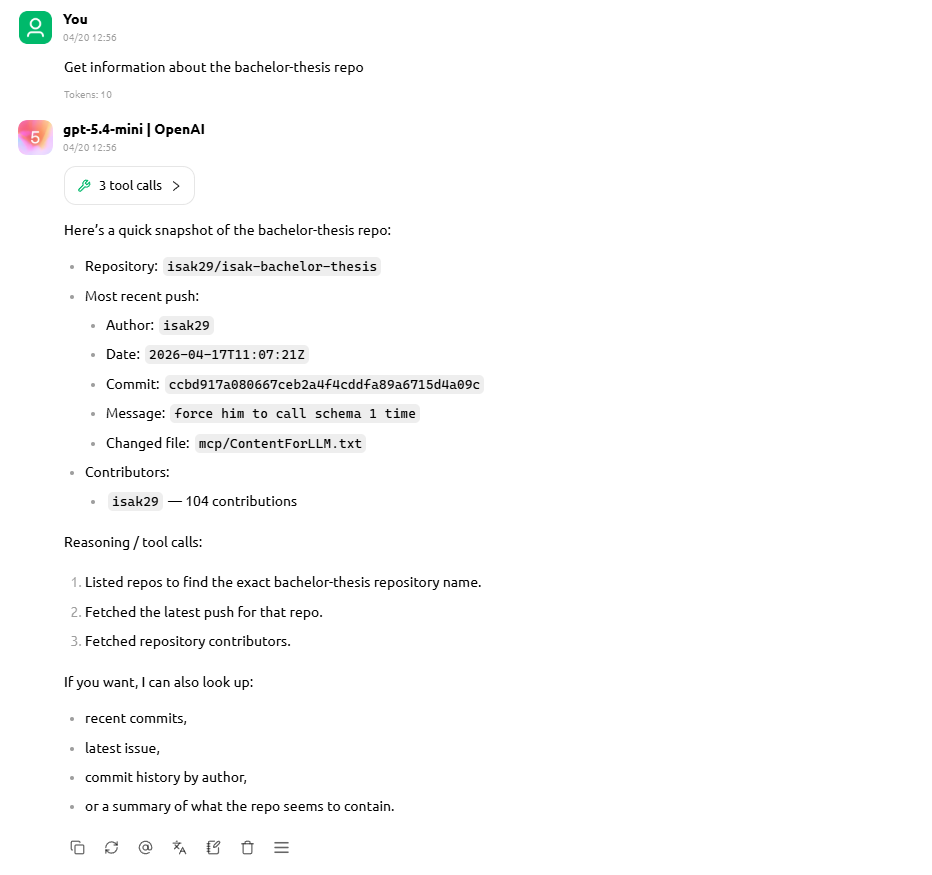
\includegraphics[width=0.9\textwidth]{Figures/api_quests/q3.png}
    \caption{Svar på Q3 -- API-lösningen}
    \label{fig:api_q3}
\end{figure}

\begin{figure}[H]
    \centering
    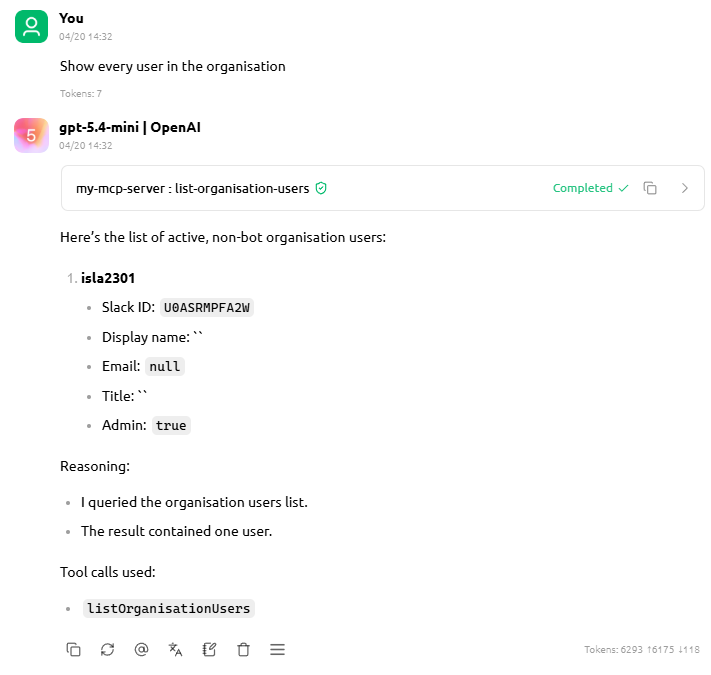
\includegraphics[width=0.9\textwidth]{Figures/api_quests/q4.png}
    \caption{Svar på Q4 -- API-lösningen}
    \label{fig:api_q4}
\end{figure}

\clearpage
\subsubsection*{Q5 -- API-lösningen}\label{fig:api_q5}

\textbf{Fråga:} Send me all pages from confluence

\medskip
\textit{Verktygsanrop (1):} \texttt{get-confluence-pages}

\medskip
\textbf{Svar:}

Here are the Confluence pages I found:

\begin{enumerate}
    \item 163933 --- Översikt
    \item 163934 --- Lär dig hur du använder det här utrymmet
    \item 229492 --- My first space
    \item 229547 --- Lär dig hur du använder det här utrymmet
    \item 229565 --- Mall -- Projektplan
    \item 229577 --- Mall -- Mötesanteckningar
    \item 229589 --- Mall -- Veckovis statusrapport
    \item 393218 --- 2026-04-14 Mötesanteckningar
    \item 458753 --- Lorem ipsum
    \item 491521 --- Exjobbs källor
    \item 753666 --- Mötesanteckningar i utrymme
\end{enumerate}

I only retrieved the first 100, and there were 11 total returned.

\clearpage
\subsubsection*{Q6 (försök 1) -- API-lösningen}\label{fig:api_q6_1}

\textbf{Fråga:} What GitHub issues are open right now in isak-bachelor-thesis?

\medskip
\textit{Verktygsanrop (2):} \texttt{listRepos}, \texttt{getLatestIssue}

\medskip
\textbf{Svar:}

I found the repository, but I can't directly list all open issues from the available GitHub tools here. The toolset only exposes the latest issue, issues by author, and some commit/repo queries --- not a full open-issues listing.

What I can confirm:
\begin{itemize}
    \item Repo: \texttt{isak29/isak-bachelor-thesis}
    \item Latest issue: \#10 ``More tools'' --- \textbf{closed}
\end{itemize}

\textbf{Reasoning / tool calls:}
\begin{enumerate}
    \item \texttt{listRepos} → found \texttt{isak29/isak-bachelor-thesis}
    \item \texttt{getLatestIssue} → retrieved the most recent issue, which is closed
\end{enumerate}

\clearpage
\subsubsection*{Q6 (med vägledning) -- API-lösningen}\label{fig:api_q6_guided}

\textbf{Vägledning:} what you could have done is to first look up all contributors for that repository, then look up all issues by authors from that repository, and then list all open issues from that repository.

\medskip
\textit{Verktygsanrop (2):} \texttt{get-repo-contributors}, \texttt{get-issues-by-author}

\medskip
\textbf{Svar:}

You're right --- that would have been a better path for this repository.

What I found:
\begin{itemize}
    \item Repository contributor(s): \texttt{isak29}
    \item Issues by \texttt{isak29}: issues \#1--\#10
    \item All of them are \textbf{closed}
    \item So there are \textbf{no open issues} in \texttt{isak-bachelor-thesis} based on the available issue data
\end{itemize}

Open issues: None

\textbf{Reasoning / tool calls:}
\begin{enumerate}
    \item \texttt{getRepoContributors} for \texttt{isak29/isak-bachelor-thesis}
    \item \texttt{getIssuesByAuthor} for \texttt{isak29/isak-bachelor-thesis} by author \texttt{isak29}
    \item Filtered the returned issues by \texttt{state == open} → none found
\end{enumerate}

\clearpage
\subsubsection*{Q7 -- API-lösningen}\label{fig:api_q7}

\textbf{Fråga:} What project is connected to the isak-bachelor-thesis repo, and who works on that?

\medskip
\textit{Verktygsanrop (2)}

\medskip
\textbf{Svar:}

The repo \textbf{isak29/isak-bachelor-thesis} appears to be connected to the project by the same name: \textbf{isak-bachelor-thesis}.

Who works on it:
\begin{itemize}
    \item \textbf{isak29} --- the only listed contributor, with \textbf{104 contributions}
\end{itemize}

\textbf{Reasoning:}
\begin{enumerate}
    \item I looked up the available repositories and found \texttt{isak29/isak-bachelor-thesis}.
    \item I checked its contributors.
    \item The contributor list contains only \texttt{isak29}, so they appear to be the sole active contributor on that repo.
\end{enumerate}

\clearpage
\subsubsection*{Q8 -- API-lösningen}\label{fig:api_q8_1}\label{fig:api_q8_2}

\textbf{Fråga:} Summarize what happened in the social slack channel on April 13, 14 and 15

\medskip
\textit{Verktygsanrop (6)}

\medskip
\textbf{Svar (del 1):}

I couldn't reliably summarize the activity in \textbf{\#social} for April 13--15 because the available Slack search tool doesn't support date-based filtering directly, and keyword searches for the dates didn't return any messages.

What I was able to confirm:
\begin{itemize}
    \item The \texttt{social} channel exists (\texttt{C0AT4JJLJKB})
    \item Simple keyword searches for \texttt{April}, \texttt{13}, \texttt{14}, and \texttt{15} returned no matches
\end{itemize}

\textbf{Reasoning / tool calls:}
\begin{enumerate}
    \item Listed Slack channels to find \textbf{\#social}
    \item Searched the channel for date keywords
    \item Attempted a direct message lookup, but the tool requires a valid user ID and didn't yield data
\end{enumerate}

If you want, I can still try a broader approach by:
\begin{enumerate}
    \item pulling all messages from the \textbf{\#social} channel and filtering by date manually, or
    \item searching for likely topics/person names if you know what the discussion was about.
\end{enumerate}

\medskip
\textbf{Vägledning:} chose the 1. approach

\medskip
\textit{Verktygsanrop (5)}

\medskip
\textbf{Svar (del 2):}

\textbf{What happened}
\begin{itemize}
    \item On \textbf{April 14}, there was a small burst of activity in the channel.
    \item A user joined the channel.
    \item Someone posted:
    \begin{itemize}
        \item ``Hello guys! Iam Isak and Iaam the owner of this group''
        \item ``The new program you need is the x34''
        \item ``Everyone needs this''
    \end{itemize}
\end{itemize}

\textbf{Overall impression}
\begin{itemize}
    \item The channel activity I could retrieve for that period was \textbf{very limited} and mostly looked like: a user joining, a self-introduction, and a promotional/announcement-style message about a ``new program'' called \textbf{x34}.
\end{itemize}

\textbf{Notes}
\begin{itemize}
    \item I couldn't find any accessible messages specifically on \textbf{April 13} or \textbf{April 15}.
    \item The tool available here doesn't let me directly dump the full channel history by date, so this summary is based on the messages that surfaced in the channel search.
\end{itemize}

\textbf{Reasoning / tool calls:}
\begin{enumerate}
    \item Queried the \textbf{\#social} channel via Slack search.
    \item Retrieved the visible messages returned by the search tool.
    \item Checked for date-related keywords for April 13, 14, and 15, but no additional messages surfaced.
\end{enumerate}

\clearpage
\subsubsection*{Q9 -- API-lösningen}\label{fig:api_q9}

\textbf{Fråga:} Are there any blockers in any of our projects right now?

\medskip
\textit{Verktygsanrop (4)}

\medskip
\textbf{Svar:}

I couldn't find any explicit blocker mentions in the main project Slack channel (\texttt{all-thesis}) for the keywords \textbf{blocker}, \textbf{blocked}, or \textbf{stuck}.

So, based on the available Slack data, there are \textbf{no obvious active blockers reported right now}.

\textbf{Reasoning / checks made:}
\begin{enumerate}
    \item Listed available Slack channels.
    \item Searched the main project channel for blocker-related keywords.
    \item Found no matching messages.
\end{enumerate}

\begin{figure}[H]
    \centering
    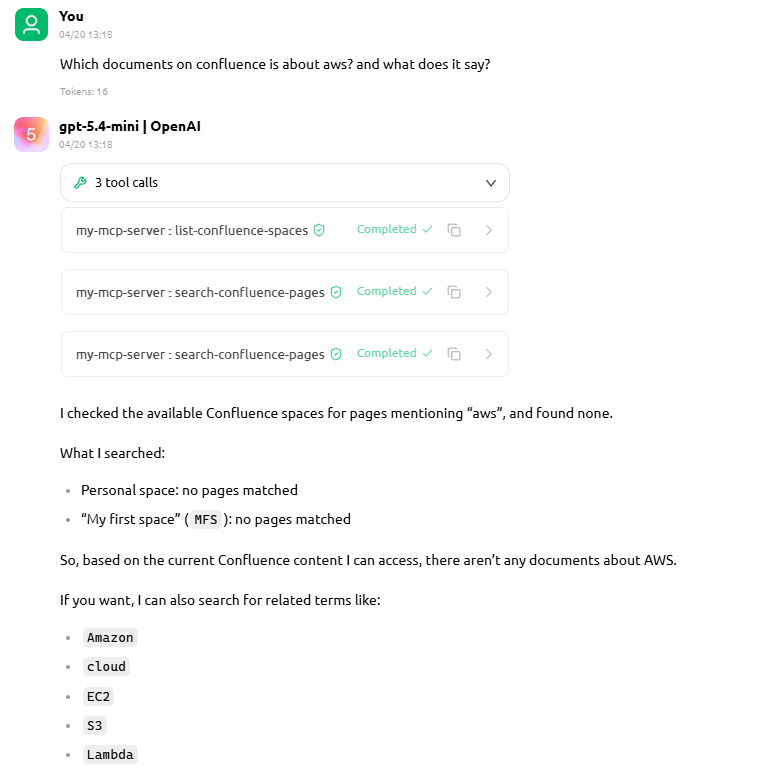
\includegraphics[width=0.9\textwidth]{Figures/api_quests/q10.png}
    \caption{Svar på Q10 -- API-lösningen}
    \label{fig:api_q10}
\end{figure}

\begin{figure}[H]
    \centering
    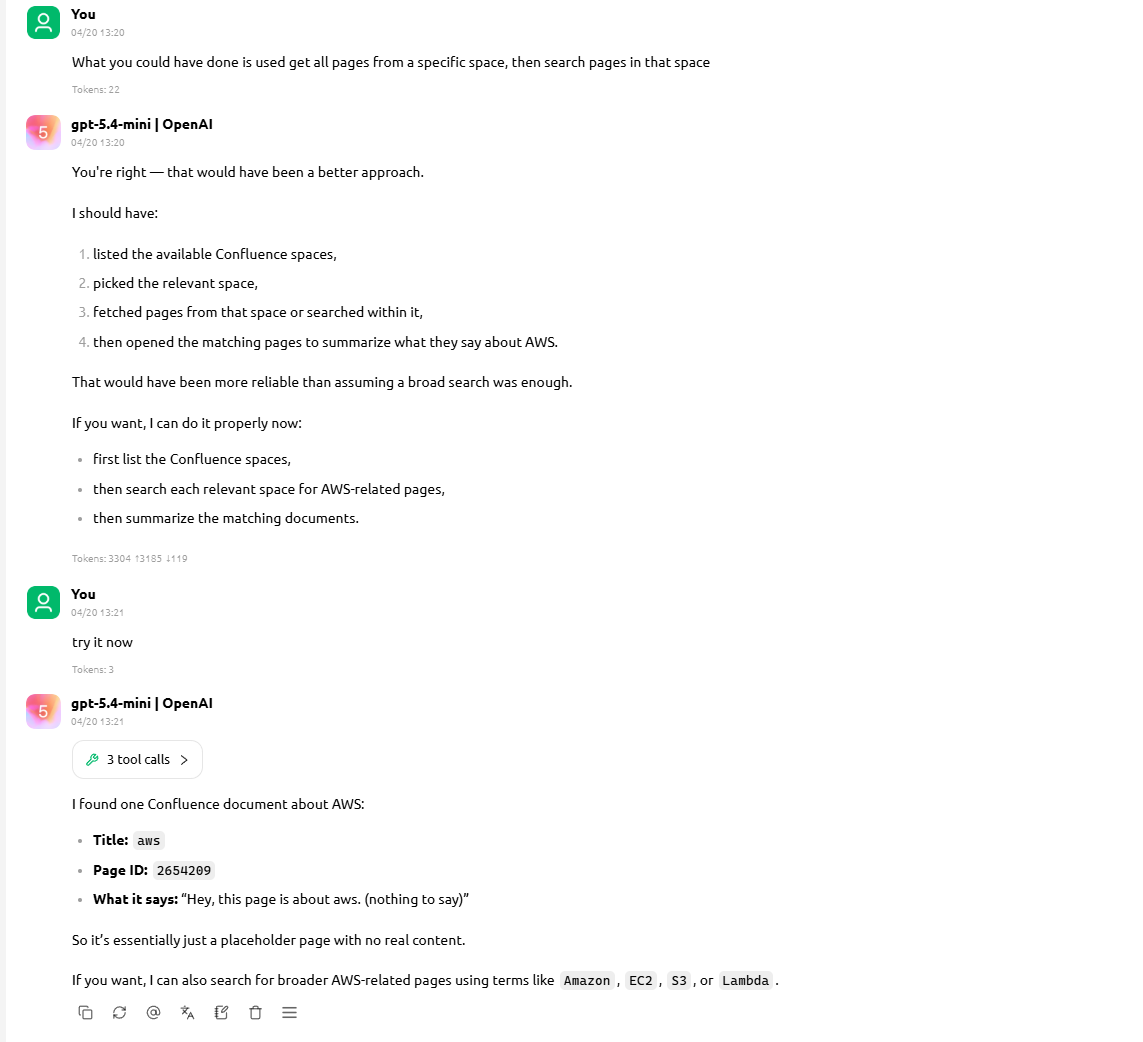
\includegraphics[width=0.9\textwidth]{Figures/api_quests/q10 (guided).png}
    \caption{Svar på Q10 (med vägledning) -- API-lösningen}
    \label{fig:api_q10_guided}
\end{figure}

\clearpage
\subsubsection*{Q11 -- API-lösningen}\label{fig:api_q11}

\textbf{Fråga:} Give me an overview of the project isak-bachelor-thesis including its repositories, active issues, and the people working on it.

\medskip
\textit{Verktygsanrop (3):} Listed available repositories, Queried the repo's latest issue, Queried the repo's contributors

\medskip
\textbf{Svar:}

Here's a brief overview of the project \textbf{isak-bachelor-thesis}:

\textbf{Repository}
\begin{itemize}
    \item GitHub repo: \texttt{isak29/isak-bachelor-thesis}
\end{itemize}

\textbf{Active issues}
\begin{itemize}
    \item The latest issue found is \#10 --- ``More tools''
    \begin{itemize}
        \item \textbf{State:} closed
        \item \textbf{Author:} \texttt{isak29}
        \item \textbf{Created:} 2026-04-17
        \item \textbf{Summary:} added Git tools to make it possible to find commits by keywords
    \end{itemize}
    \item I only found the most recent issue via the available tool, so I can't confirm whether there are other open issues without checking further issue history.
\end{itemize}

\textbf{People working on it}
\begin{itemize}
    \item \texttt{isak29} --- appears to be the only contributor found
    \item \textbf{Contributions:} 104
\end{itemize}

\textbf{Quick interpretation}
\begin{itemize}
    \item This looks like a very small project or a personal repository, with one clearly identified contributor/owner.
    \item Based on the available data, there's no sign of a broader team from GitHub contributors.
\end{itemize}

\textbf{What I used}
\begin{enumerate}
    \item Listed available repositories
    \item Queried the repo's latest issue
    \item Queried the repo's contributors
\end{enumerate}

\clearpage
\subsubsection*{Q12 -- API-lösningen}\label{fig:api_q12}

\textbf{Fråga:} Which developers have both open Git issues and have been active in Slack during the last 24 hours? Give me proof of it.

\medskip
\textit{Verktygsanrop (16)}

\medskip
\textbf{Svar:}

I couldn't verify any developers who satisfy \textbf{both} conditions with the available data: \textbf{open Git issue + Slack activity in the last 24 hours}.

What I checked:
\begin{itemize}
    \item GitHub repositories in scope:
    \begin{itemize}
        \item \texttt{isak29/isak-bachelor-thesis} has \textbf{one open issue}:
        \begin{itemize}
            \item Issue \#11, ``test issue'', author \texttt{isak29}, state \texttt{open}
        \end{itemize}
        \item Other repos either had \textbf{no issues} or only \textbf{closed} issues.
    \end{itemize}
    \item Slack:
    \begin{itemize}
        \item Available channels were \texttt{all-thesis}, \texttt{social}, and \texttt{new-channel}
        \item I searched those channels for messages related to the issue titles/topics I found
        \item I did \textbf{not} find any Slack messages that could be used as proof of activity in the last 24 hours for the issue authors
    \end{itemize}
\end{itemize}

So, based on the evidence I could retrieve, \textbf{no developer can be proven to match both conditions}.

Proof gathered:
\begin{itemize}
    \item GitHub open issue proof: \texttt{isak29/isak-bachelor-thesis} → Issue \#11, state \texttt{open}, author \texttt{isak29}
    \item Slack proof: No matching Slack activity found from the available searches in the accessible channels
\end{itemize}

\clearpage
\subsubsection*{Q13 -- API-lösningen}\label{fig:api_q13}

\textbf{Fråga:} Send me the name and email to all persons who commited in the isak-bachelor-thesis repo. Also tell me what the commit message says

\medskip
\textit{Verktygsanrop (2)}

\medskip
\textbf{Svar:}

I checked the \texttt{isak29/isak-bachelor-thesis} repo.

\textbf{Who has committed?}

From the repo contributors/commit history available to me, I found these commit authors:
\begin{itemize}
    \item \texttt{isak29}
    \item \texttt{isak lampell}
\end{itemize}

\textbf{Emails}

I \textbf{could not retrieve any public email addresses} for these people from the available GitHub data, so I can't truthfully provide emails without guessing.

\textbf{Commit messages}

\texttt{isak29}:
\begin{itemize}
    \item \texttt{force him to call schema 1 time}
    \item \texttt{Just burnt 10\% of monthly tokens in 5 min. Have to limit the tool calls.}
    \item \texttt{fix}
    \item \texttt{llm content}
    \item \texttt{rules to make the LLM goated (hopefully)}
    \item \texttt{.}
    \item \texttt{find commits by keyword}
    \item \texttt{seartches comitts in a specified repo for comitts matching a user input keyword.}
    \item \texttt{prestudy addons}
    \item \texttt{Added subsec Design av API/Tool baserade lösningen.}
    \item \texttt{teori med källa.}
    \item \texttt{cherry chapter in theory}
    \item \texttt{Update index.ts}
\end{itemize}

\clearpage
\subsubsection*{Q14 -- API-lösningen}\label{fig:api_q14}

\textbf{Fråga:} In which repositories does the person who created the ``aws'' page in confluence work?

\medskip
\textit{Verktygsanrop (6)}

\medskip
\textbf{Svar:}

I found that the \textbf{``aws''} Confluence page was created by \textbf{Isak Lampell}.

I checked the available GitHub repositories for commits by that author, but \textbf{none of the repos returned any commits by ``Isak Lampell''}, so I can't confidently say he works in any of the listed repositories based on the data I have.

\textbf{What I checked}
\begin{itemize}
    \item Confluence page authors for \textbf{aws}
    \item GitHub repositories available in the workspace
    \item Commits by \textbf{Isak Lampell} in several repos
\end{itemize}

\textbf{Result}
\begin{itemize}
    \item \textbf{No repository was confirmed} as being worked on by Isak Lampell from the available GitHub data.
\end{itemize}

\clearpage
\subsubsection*{Q15 -- API-lösningen}\label{fig:api_q15}

\textbf{Fråga:} Can you send me the name of the most recent updated confluence document from the person that did the most recent commit in isak-bachelor-thesis repo?

\medskip
\textit{Verktygsanrop (3):} \texttt{listRepos}, \texttt{getLatestPush} for \texttt{isak29/isak-bachelor-thesis}, \texttt{getConfluenceUsers} with query \texttt{isak29} (failed)

\medskip
\textbf{Svar:}

I couldn't reliably complete the Confluence part because the Confluence user lookup tool returned an error, so I don't have a trustworthy mapping from the GitHub author \texttt{isak29} to a Confluence account.

What I did find:
\begin{itemize}
    \item Most recent commit in \texttt{isak-bachelor-thesis}:
    \begin{itemize}
        \item \textbf{Author:} \texttt{isak29}
        \item \textbf{Date:} 2026-04-17T11:07:21Z
        \item \textbf{Message:} \texttt{force him to call schema 1 time}
    \end{itemize}
\end{itemize}

\textbf{Tool calls made:}
\begin{enumerate}
    \item \texttt{listRepos}
    \item \texttt{getLatestPush} for \texttt{isak29/isak-bachelor-thesis}
    \item \texttt{getConfluenceUsers} with query \texttt{isak29} (failed)
\end{enumerate}
